\documentclass[wide,a4paper,titlepage,12pt] {article}
\usepackage{polski}
\usepackage[utf8]{inputenc}
\usepackage{listings}
\usepackage{slashbox}
\usepackage[table]{xcolor}
\usepackage{graphicx,pdflscape}
\usepackage{placeins}


\title{Układy cyfrowe i systemy wbudowane}
\author{Tymon Tobolski (181037)\\ Jacek Wieczorek (181043)}

% Title page layout (fold)
\makeatletter
\renewcommand{\maketitle}{
\begin{titlepage}
  \begin{center}
    \vspace*{3cm}
    \LARGE \@title \par
    \vspace{2cm}
    \textit{\small Autor:}\par
    \normalsize \@author\par \normalsize
    \vspace{3cm}
    \textit{\small Prowadzący:}\par
    Dr inż. Jarosław Sugier \par
    \vspace{2cm}
    Wydział Elektroniki\\ III rok\\ Pn 14.15 - 16.00\par
    \vspace{4cm}
    \small \@date
  \end{center}
\end{titlepage}
}
\makeatother
% Title page layout (end)



\begin{document}
\maketitle
  \section{Cel laboratorium}

  \section{Zadanie nr 1}
  Celem zadania było zamodelowanie układu licznika wykonującego sekwencję 2 0 1 3 4 5 6 7, przetestowanie jego działania w symulatorze, a następnie uruchomienie go na płycie $ZL-9572$. Układ miał za zadanie wyświetlać na diodach LED kolejne cyfry sekwencji (w reprezentacji binarnej) po naciśnięciu przycisku. Drugi przycisk służył do resetowania stanu licznika do pozycji początkowej. Ponadto ćwiczenie zakładało sprawdzenie czasu reakcji przerzutnika na zmianę sygnału zegara za pomocą symulatora. Do realizacji tego układu zostały wykorzystane trzy przerzutniki typu D sterowane jednym sygnałem zegarowym. Dodatkowym zadaniem przy realizacji tego układu było sterowanie licznikiem za pomocą Rotora komunikacji szeregowej z komputerem za pomocą portu $RS232$.

  W celu wyznaczenia odpowiednich kombinacji syngałów dla wejść przerzutników zostosowana została metoda siatek Karnaugh.

  \paragraph{}

	  \begin{center}

	  \begin{tabular}{|c|c|c||c|c|c|}
			\hline
			$Q_{2}$ & $Q_{1}$ & $Q_{0}$ & $Q_{2}'$ & $Q_{1}'$ & $Q_{0}'$ \\
			\hline
      0 & 0 & 0 & 0 & 0 & 1 \\
      0 & 0 & 1 & 0 & 1 & 1 \\
      0 & 1 & 0 & 0 & 0 & 0 \\
      0 & 1 & 1 & 1 & 0 & 0 \\
      1 & 0 & 0 & 1 & 0 & 1 \\
      1 & 0 & 1 & 1 & 1 & 0 \\
      1 & 1 & 0 & 1 & 1 & 1 \\
      1 & 1 & 1 & 0 & 1 & 0 \\
      \hline
	  \end{tabular}
	 \\ Tabela zmiany stanu przerzutników
	  \end{center}

    \begin{center}
      \begin{tabular}{|c|c|c|c|c|}
        \hline
        \backslashbox{$Q_{0}$}{$Q_{2}$$Q_{1}$} & 00 & 01 & 11 & 10 \\ \hline
        0 & 0 & 0 & \cellcolor[gray]{0.8} 1 & \cellcolor[gray]{0.8} 1 \\ \hline
        1 & 0 & \cellcolor[gray]{0.8} 1 & 0 & \cellcolor[gray]{0.8} 1 \\ \hline
      \end{tabular}
      \\ $Q_{2}'$ = $Q_{2} \bar{Q_{0}} + Q_{2} \bar{Q_{1}} + \bar{Q_{2}} Q_{1} \bar{Q_{0}}$
    \end{center}

    \begin{center}
      \begin{tabular}{|c|c|c|c|c|}
        \hline
        \backslashbox{$Q_{0}$}{$Q_{2}$$Q_{1}$} & 00 & 01 & 11 & 10 \\ \hline
        0 & 0 & 0 & \cellcolor[gray]{0.8} 1 & 0 \\ \hline
        1 & \cellcolor[gray]{0.8} 1 & 0 & \cellcolor[gray]{0.8} 1 & \cellcolor[gray]{0.8} 1 \\ \hline
      \end{tabular}
      \\ $Q_{1}'$ = $Q_{2} Q_{1} + \bar{Q_{1}} Q_{0}$
    \end{center}

    \begin{center}
      \begin{tabular}{|c|c|c|c|c|}
        \hline
        \backslashbox{$Q_{0}$}{$Q_{2}$$Q_{1}$} & 00 & 01 & 11 & 10 \\ \hline
        0 & \cellcolor[gray]{0.8} 1 & 0 & \cellcolor[gray]{0.8} 1 & \cellcolor[gray]{0.8} 1 \\ \hline
        1 & \cellcolor[gray]{0.8} 1 & 0 & 0 & 0 \\ \hline
      \end{tabular}
      \\ $Q_{0}'$ = $Q_{2} \bar{Q_{0}} + \bar{Q_{2}} \bar{Q_{1}}$
    \end{center}



	\paragraph{}

	\begin{figure}[htbp]
	 		\begin{center}
         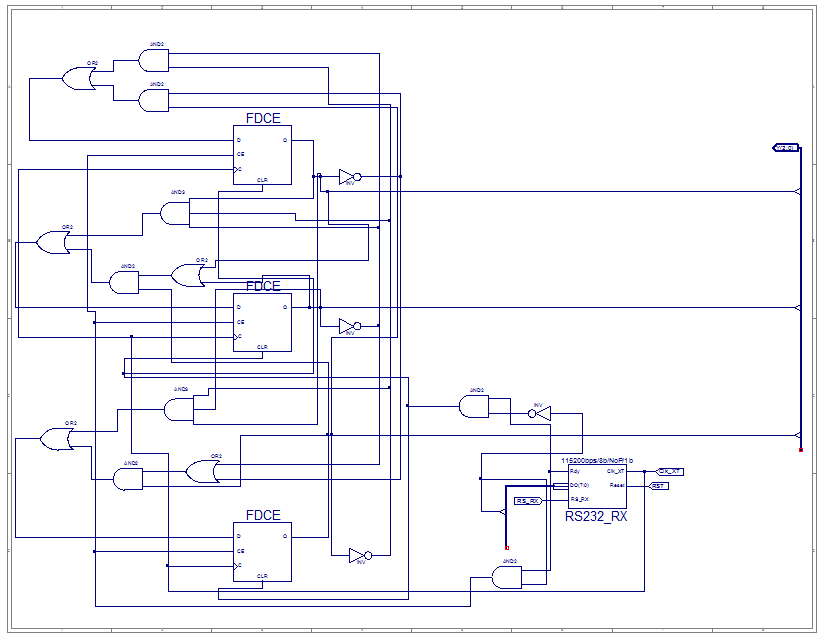
\includegraphics[scale=0.7]{Capture.PNG}
      \caption{Schemta układu}
     \end{center}
  \end{figure}

  \paragraph{}
  Następnym etapem ćwiczenia było napisanie testów, oraz odpowiednie zmodyfikowanie pliku \textit{ZL-9572.ucf} pozwalające na zasymulowanie układu i wyświetlenie wyników na diodach.
	\\ \\ \\
	\paragraph{}
	Fragment zmodyfikowanego pliku \textit{ZL-9572.ucf} :
	\lstinputlisting[language=Vhdl]{ZL-9572.ucf}

	\paragraph{}
	Układ został najpierw zasymulowany i sprawdzony za pomocą programu ModelSim, a następnie wgrany do urządzenia i przetestowany na układzie scalonym.

		\paragraph{}
	Testy w języku VHDL:
	\lstinputlisting[language=Vhdl]{code4.txt}
		\paragraph{}
		\paragraph{}

	Następnie za pomocą symulatora ModelSim został sprawdzony czas reakcji przerzutnika na zmiane sygnału zegara co widać na Rysunku 2.

		\paragraph{}

		\begin{figure}[htbp]
	 		\begin{center}
         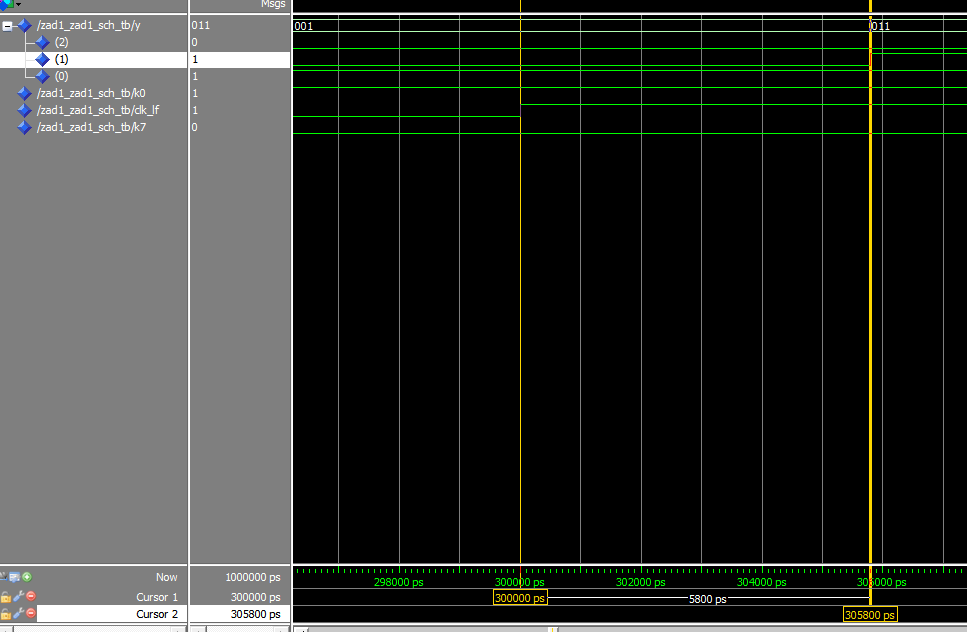
\includegraphics[scale=0.4]{screen.png}
      \caption{Prezentacja czasu reakcji przerzutnika}
     \end{center}
  \end{figure}

  \paragraph{}
  Podłączenie rotora pozwalało na inkrementacje sekwencji licznika za pomocą obrotu rotorem w prawo oraz powrót do wartości początkowej za pomocą obrotu w lewo.

  Po podłączeniu układu RS232 możliwe stało się sterowanie licznikiem za pomocą komputera podłączonego do układu poprzez port szeregowy. W celu uproszczenia dekodera danych w układzie licznik zwiększał się przy wysłaniu z terminala dowolnej małej litery alfabetu, a resetował się przy wysłaniu dowolnej dużej litery. Takie założenia pozwoliły na maksymalne uproszczenie układu dekodującego do dwóch bramek, ponieważ w kodzie ASCII każda mała litera alfabetu ma wartość 5-tego bitu równą 1, natomiast każda duża litera ma w tym miejscu wartość 0.


  \paragraph{}
  \newpage
  \section{Wnioski}
  Edytor ECS pozwala na modelowanie bardziej skomplikowanych układów za pomocą składania ich z prostszych, wcześniej przygotowanych elementów (np. Rotor, RS232). ozwala to skupić się na istocie problemu, a nie na szczegółach technicznych np. komunikacji z komputerem. Układ we wszystkich wersjach (przyciski, rotor, rs232) działał zgodnie z założeniami.

\end{document}